\documentclass[11pt]{article}
\usepackage[utf8]{inputenc}\usepackage[T1]{fontenc}\usepackage{lmodern}
\usepackage[spanish,es-nodecimaldot]{babel}\usepackage[margin=1in]{geometry}
\usepackage{amsmath,amssymb,amsthm,booktabs,graphicx,array,xcolor}
\usepackage[round]{natbib}\usepackage[colorlinks=true,allcolors=blue!50!black]{hyperref}
\newtheorem{proposition}{Proposición}\newtheorem{assumption}{Supuesto}
\setlength{\parindent}{0pt}\setlength{\parskip}{5pt}
\newcommand{\q}{q}\newcommand{\wv}{w^V}\newcommand{\vL}{v_L}\newcommand{\vM}{v_M}
\title{Verificación heterogénea y acceso a la IA\\\large Selección intermedia en una economía de conocimiento}
\author{Sofía Belén Vásquez García\\\small Universidad del Pacífico, AI and Economic Modeling\\\small\url{https://github.com/sbvasquezg-ux/ai-project}}
\date{26 de octubre de 2026}
\begin{document}\maketitle
\begin{abstract}\noindent
Estudio si un gasto real de validación que cae con el conocimiento modifica quién usa una IA no autónoma. Extiendo la actividad humano--IA de Ide y Talamàs (2025), conservando su tecnología de ayuda y agregando $c(z)=\kappa(1-z)$. Con cómputo ocioso, la libre entrada determina $w^V=a-c$ entre usuarios. El resultado principal caracteriza un equilibrio de tres tipos: bajo desigualdades explícitas sobre ofertas netas y suficiente masa experta, solo el tipo intermedio adopta, mientras la base trabaja con expertos humanos. Una prueba por factibilidad, beneficios y complementariedad establece asignación y salarios únicos en ese régimen. Un ejemplo racional y programas lineales verifican el resultado. Mallas de una distribución uniforme también presentan adopción intermedia, pero no prueban existencia, unicidad ni convergencia del equilibrio continuo. Las dos proposiciones se comprueban en Lean, incluida la existencia y unicidad del equilibrio finito; la revisión manuscrita de la autora sigue pendiente.
\end{abstract}
\section{Introducción}
El acceso técnico al conocimiento de una IA no implica que todos los trabajadores puedan incorporarla con el mismo costo. Si revisar y documentar su uso exige un gasto mayor a quienes tienen menos conocimiento, la tecnología puede resultar económicamente atractiva para tipos que no están en la base. Esa intuición compite con el costo de oportunidad: los más preparados también disponen de mejores opciones laborales. La pregunta es si esta fricción puede desplazar la adopción directa hacia tipos intermedios cuando salarios y asignaciones se ajustan.

La Proposición 6 de \citet{ide2025}, p. 27 de arXiv v11, caracteriza la IA no autónoma sin esta fricción. Con adopción, los usuarios directos están en la base del conocimiento. Aquí el aporte formal es una caracterización suficiente en la especialización de tres tipos prevista en la propuesta inicial, con prueba completa de equilibrio. El continuo uniforme conserva el papel de ejercicio numérico. El resultado no atribuye un error al artículo base ni demuestra que la selección intermedia ocurra para cualquier costo decreciente.

La contribución consta de una condición salarial local y un resultado de asignación. El segundo requiere comparar todas las actividades, y no solo resolver la FOC. La distinción es esencial: una diferencia positiva frente al salario anterior a la IA puede desaparecer cuando cambian los precios. Las pruebas y los chequeos siguientes mantienen esa separación.
\newpage
\section{Baseline y literatura relacionada}
\textbf{Resultado que se extiende.} \emph{Artificial Intelligence in the Knowledge Economy} está publicado en \emph{Journal of Political Economy}, 133(12), 3762--3800. Uso la paginación de arXiv:2312.05481v11: tecnología y beneficios en la sección 3.1, p. 12, e IA no autónoma en la sección 6, con Proposición 6 en p. 27. Escribo $a$ en lugar de $z_{\mathrm{AI}}$, $w^0$ por el salario inicial $w$ y $w^N$ por el salario $w^\star$ con copiloto sin costo. Cuando $a>w^0(0)$, el baseline tiene adopción desde la base y $w^N=a$ entre usuarios, con $r=0$; cuando $a\leq w^0(0)$, no hay adopción.

La sección 2.6 del apéndice enlazado por el autor demuestra el ordenamiento mediante los Lemas 2.7--2.8 (pp. impresas 21--23). Su argumento utiliza salarios iguales entre usuarios. El gasto por tipo introduce una oferta inclinada y obliga a revisar esa comparación. El capítulo 5 (pp. 64--74) aborda otras consecuencias y cómputo escaso \citep{appendix}. El registro en \texttt{proposal/literature-search.md} documenta la revisión de v1--v12: la v7 estudia otra formulación de no autonomía; v8--v10 contienen la selección inferior como Proposición 7; v11--v12 la presentan como Proposición 6. No se intercambian sus pruebas automáticamente.

\textbf{Verificación y conocimiento.} La idea general de que validar cuesta y depende de la experiencia ya tiene antecedentes. \citet{catalini}, preprint, relaciona costo de verificación, experiencia y remuneración experta; mayor eficiencia no garantiza menor gasto si aumenta el salario. \citet{quispe2026}, preprint v2, supone costos de especificación y verificación decrecientes con habilidad y familiaridad. Su banda de activación selecciona lenguajes para un desarrollador. Aquí la selección opera sobre tipos humanos y sus ocupaciones, con salarios que vacían el mercado.

\textbf{Jerarquías y supervisión.} \citet{xu2025}, preprint v1, incorpora validación gerencial que consume tiempo y elimina alucinaciones. La v2 de marzo de 2026 amplía el análisis a modos de automatización y aumento de capacidad en distintas capas \citep{xu2026}. Mi fricción mantiene la probabilidad de éxito y el tiempo de ayuda del baseline; es gasto en bien final. \citet{turing}, documento de trabajo anunciado como aceptado en \emph{Journal of Human Capital} por la web del autor, estudia conocimiento multidimensional y sinergias, otro margen de heterogeneidad.

La búsqueda inicial consultó Scholar, ``Citado por'' y \texttt{verification} entre citantes, arXiv y apéndices; Semantic Scholar respondió 429. El 26 de octubre se revalidaron las fichas de los antecedentes y se identificó la v2 de Xu y coautores, que no se había discutido en el topic. No se afirma una revisión exhaustiva ni originalidad del concepto de verificación: la contribución propuesta es el régimen competitivo específico caracterizado aquí.
\newpage
\section{Modelo y alcance de la extensión}
\begin{assumption}[Tecnología e información]\label{ass:tech}
Los tipos observables son $z\in[0,1]$, la masa humana total es uno y los problemas tienen dificultad uniforme. Cada trabajador genera una unidad de problemas por período. Un solver con conocimiento $s>z$ permite producto esperado $s$ por trabajador y dedica $b(z)=h(1-z)$ de su tiempo, con $0<h<1$. Solo hay dos niveles, competencia y libre entrada. Para la comparación continua del artículo se conserva $0<h<h_0(G)$ y densidad positiva continua de $G$.
\end{assumption}
\begin{assumption}[IA y gasto real]\label{ass:ai}
La IA no autónoma solo asesora; tiene capacidad fija $a\in(0,1)$ y puede ayudar a $z\leq a$. El gasto obligatorio $c(z)\geq0$ por trabajador y período se paga en bien final y no consume tiempo ni altera éxito. En el ejercicio principal $c(z)=\kappa(1-z)$, $\kappa\geq0$. El costo constante es una comparación separada.
\end{assumption}
\begin{assumption}[Cómputo]\label{ass:compute}
La dotación $\mu>h$ es exógena y el cómputo ocioso tiene renta cero. Como su demanda es $\int b(z)x(dz)\leq h$, resulta $r=0$.
\end{assumption}
Una unidad de IA atiende $n(z)=1/b(z)$. La firma elige el tipo contratado tomando salarios y renta como dados:
\begin{equation}\label{eq:firm}
\max_{0\leq z\leq a}\Pi^V(z)=n(z)[a-\wv(z)-c(z)]-r.
\end{equation}
Defino la oferta neta $\q(z)=a-c(z)$. La comparación inicial es $\Delta^0(z)=\q(z)-w^0(z)$; no es una condición que determine el nuevo equilibrio.

\begin{assumption}[Especialización finita]\label{ass:finite}
Para el resultado global se reemplaza la distribución continua por la terna $(0,m,H)$, con $0<m<H<1$ con masas positivas $\alpha,\beta,\gamma$, cuya suma es uno. Se conservan tecnología, información, actividades y fricción de los Supuestos 1--3. Para el resultado de tres tipos se exige $m<a$ y las condiciones adicionales de la Proposición 2.
\end{assumption}
Este cambio de distribución es explícito: corresponde al plan B de la propuesta. El teorema finito no se presenta como una prueba del continuo. Las masas son divisibles; una fracción de cada tipo puede trabajar en cada ocupación.

En una población finita general, $d_i$ es masa independiente, $x_i$ masa de usuarios de IA y $y_{ij}$ trabajadores $i$ asistidos por humanos $j>i$. Un equilibrio requiere recursos factibles, vaciado humano, salarios que impidan beneficios positivos y beneficio cero en actividades utilizadas. La normalización por trabajador deja la desigualdad humano--humano $w_i+b_iw_j\geq z_j$. Este salario es remuneración por tiempo humano, no una elección unilateral de la firma.
\newpage
\section{Resultado local y derivación}
\begin{proposition}[FOC y salario de una actividad usada]\label{prop:local}
Bajo los Supuestos 1--3, sean $0<z<a<1$ y $w^V,c$ diferenciables en un entorno de $z$. Si $z$ maximiza localmente el beneficio de \eqref{eq:firm}, entonces
\begin{equation}\label{eq:foc}
w^{V\prime}(z)+c'(z)=\frac{a-w^V(z)-c(z)}{1-z}.
\end{equation}
Si además la actividad tiene beneficio cero, el cociente es $hr$. Con $r=0$, $w^V(z)=a-c(z)$. Si la actividad es usada en un intervalo abierto y $c(z)=\kappa(1-z)$, entonces $w^{V\prime}(z)=\kappa$ en ese intervalo.
\end{proposition}
\begin{proof}
Como $h>0$ y $z<1$, todos los denominadores son positivos. La regla de la cadena y la derivación de un recíproco dan
\[
n'(z)=\frac{1}{h(1-z)^2},\qquad
\frac{n'(z)}{n(z)}=\frac{1}{1-z}.
\]
La regla del producto, manteniendo $a,h,r$ fijos, implica
\[
\Pi^{V\prime}(z)=n'(z)[a-w^V(z)-c(z)]-n(z)[w^{V\prime}(z)+c'(z)].
\]
La interioridad y el máximo local permiten aplicar la condición de Fermat: $\Pi^{V\prime}(z)=0$. Dividir por $n(z)>0$ y sustituir $n'/n$ produce \eqref{eq:foc}. Por otra parte, beneficio cero significa
\[
 n(z)[a-w^V(z)-c(z)]=r
 \quad\Longrightarrow\quad a-w^V(z)-c(z)=rh(1-z).
\]
Sustituyendo en \eqref{eq:foc}, $w^{V\prime}+c'=hr$. Si $r=0$, la igualdad de beneficio cero entrega la identidad de nivel. Sobre un intervalo usado se puede derivar esa identidad: $w^{V\prime}=-c'=\kappa$.
\end{proof}
El primer término de la derivada valora mayor escala; el segundo recoge el costo de cambiar de tipo. La igualdad salarial procede de beneficio cero, incluso sin optimalidad interior. La pendiente, en cambio, necesita una identidad válida alrededor del punto. No se deduce la derivada de una igualdad que solo valga en un tipo aislado.

La FOC tampoco es suficiente para un máximo estricto. Sustituir el salario de beneficio cero en el beneficio puede generar indiferencia entre tipos. En un extremo del dominio, las condiciones necesarias son unilaterales: $\Pi^{V\prime}(0)\leq0$ o $\Pi^{V\prime}(a)\geq0$, cuando existen las derivadas correspondientes.

Un detalle útil para interpretar la parametrización es $n(z)c(z)=\kappa/h$: el gasto por unidad de IA es constante en esta forma lineal. Aun así, la oferta salarial por trabajador es $a-\kappa+\kappa z$. La selección requiere comparar esa oferta con las actividades humanas y los recursos, que no son constantes en $z$.
\newpage
\section{Resultado de equilibrio: adopción intermedia}
Para la población del Supuesto 4, escribo
\[
 b_M=h(1-m),\quad \vL=H(1-h),\quad \vM=H(1-b_M),\quad
 q_L=a-\kappa,\quad q_M=a-\kappa(1-m).
\]
Si $H\leq a$, también $q_H=a-\kappa(1-H)$. Las cantidades $\vL,\vM$ son salarios financiados al combinar cada tipo inferior con expertos de salario $H$.

\begin{proposition}[Régimen intermedio de tres tipos]\label{prop:middle}
Bajo los Supuestos 1--4, supóngase
\begin{align}
 &\gamma>h\alpha+b_M\beta,\qquad \vM>m,\label{eq:surplus}\\
 &q_L<\vL,\qquad q_M>\vM,\label{eq:offers}\\
 &q_H<H\quad\text{si }H\leq a.\label{eq:high}
\end{align}
Sin IA existe un único equilibrio en asignaciones y salarios: los tipos $L,M$ trabajan con expertos $H$, el resto de $H$ produce de forma independiente, y $w^0=(\vL,\vM,H)$. Con validación heterogénea existe un único equilibrio en asignaciones y salarios:
\begin{equation}\label{eq:prices3}
 (w^V_L,w^V_M,w^V_H)=(\vL,q_M,H).
\end{equation}
Solo $M$ usa IA: $x_M=\beta$, $x_L=x_H=0$. La base trabaja con expertos, $y_{LH}=\alpha$, y $d_H=\gamma-h\alpha$; las demás actividades son nulas. El producto neto aumenta respecto de la economía sin IA en
\begin{equation}\label{eq:gain}
 Y^V-Y^0=\beta(q_M-\vM)>0.
\end{equation}
\end{proposition}
Las condiciones tienen interpretación económica. La primera deja expertos independientes incluso antes de la IA; así su salario se fija en $H$. La segunda hace rentable emplear al tipo medio como trabajador antes de IA. Las ofertas netas descartan la IA para la base y la prefieren para el tipo intermedio. La última evita que la IA absorba a los expertos necesarios para sostener la alternativa humana.

La conclusión no supone que los adoptantes ya sean intermedios. Los salarios y las actividades se construyen a partir de primitivas, se comprueba que ningún desvío da beneficio positivo y se demuestra que los mercados se vacían. Las desigualdades estrictas definen un régimen; en sus fronteras puede haber indiferencia y múltiples asignaciones. La proposición no caracteriza todos los regímenes paramétricos.

En esta especialización se reemplaza el supuesto de densidad continua. El resultado demuestra la posibilidad de selección intermedia en la economía discreta extendida. La propiedad equivalente para todas las distribuciones continuas admisibles permanece abierta; la sección numérica investiga una de ellas.
\newpage
\subsection{Prueba de la Proposición 2}
\begin{proof}
\textbf{1. Economía sin IA.} Propongo $y_{LH}=\alpha$, $y_{MH}=\beta$ y $d_H=\gamma-h\alpha-b_M\beta>0$. Se utilizan exactamente las masas de cada tipo. A salarios $(\vL,\vM,H)$, las actividades $LH,MH$ y la producción independiente de $H$ tienen beneficio cero. Los tipos inferiores no prefieren producción independiente porque $\vL>0$ y $\vM>m$. La actividad $LM$ tampoco es rentable:
\begin{equation}\label{eq:slack}
 \vL+h\vM-m=(\vM-m)+Hh(1-h)(1-m)>0.
\end{equation}
Se verifican todas las actividades de dos niveles. Cómputo no usado y $r=0$ satisfacen su mercado.

\textbf{2. Equilibrio con IA.} Propongo las actividades y salarios de \eqref{eq:prices3}. La base ocupa masa $\alpha$ y demanda $h\alpha$ expertos; $M$ usa masa $\beta$ en IA; el remanente $\gamma-h\alpha>0$ de expertos produce solo. La demanda de cómputo es $b_M\beta<h<\mu$, de modo que $r=0$ es compatible con ociosidad.

\textbf{3. Ausencia de beneficios positivos.} $LH$ tiene costo $\vL+hH=H$ y beneficio cero. La IA de $M$ tiene producto neto $q_M=w^V_M$ y también beneficio cero. $H$ independiente recibe $H$. La actividad $MH$ tiene holgura $q_M+b_MH-H=q_M-\vM>0$. La actividad $LM$ tiene holgura $\vL+hq_M-m>\vL+h\vM-m>0$ por \eqref{eq:slack}. $L,M$ independientes son estrictamente menos rentables que sus salarios. La IA de $L$ no cubre $\vL$ porque $q_L<\vL$; si $H$ es elegible, su IA tampoco cubre $H$. Así se han enumerado todas las actividades posibles. Recursos, salarios y beneficio cero prueban existencia competitiva.

\textbf{4. Unicidad.} Multiplicar cada restricción de no beneficio por su actividad y sumar da, para cualquier asignación factible, producto neto no mayor que la masa salarial del salario candidato. La asignación construida alcanza esa cota. Cualquier otro equilibrio también alcanza el máximo: aplicar sus restricciones salariales a una asignación óptima y usar vaciado y beneficio cero produce las desigualdades opuestas. En un óptimo, ninguna actividad con holgura estricta bajo el salario candidato puede utilizarse. Solo quedan $LH$, IA de $M$ e independientes $H$; los recursos fijan sus masas como arriba. Como las tres tienen masa positiva, sus igualdades de beneficio cero fijan sucesivamente $w_H=H$, $w_L=\vL$ y $w_M=q_M$. El mismo argumento, con actividades $LH,MH,H$ independientes, prueba unicidad sin IA.

\textbf{5. Producto.} Las expresiones factibles son
\[
Y^0=(\alpha+\beta)H+(\gamma-h\alpha-b_M\beta)H,
\quad Y^V=\alpha H+\beta q_M+(\gamma-h\alpha)H.
\]
Restar y usar $\vM=H(1-b_M)$ da \eqref{eq:gain}.
\end{proof}
\newpage
\section{Un equilibrio racional que satisface las condiciones}
Fijo los mismos $h,a,\kappa$ del topic, pero una población explícita de tres tipos:
\[
h=\tfrac12,\quad a=\tfrac{22}{25}=0.88,\quad\kappa=\tfrac{53}{100}=0.53,
\]
\[
(z_L,z_M,z_H)=(0,\tfrac14,\tfrac{19}{25}),
\quad(\alpha,\beta,\gamma)=(\tfrac14,\tfrac25,\tfrac7{20}).
\]
Las necesidades de expertos son $h\alpha=0.125$ y $b_M\beta=0.15$, por lo que $0.35>0.275$. Los salarios humanos son $\vL=0.38$, $\vM=0.475>m=0.25$. Las ofertas netas son
\[
 q_L=0.35<0.38,\quad q_M=0.4825>0.475,\quad q_H=0.7528<0.76.
\]
Todas las desigualdades de la proposición son estrictas. El script \texttt{code/verify.py} genera un certificado racional. Evalúa cada recurso, desigualdad salarial e igualdad en actividades usadas con SymPy; una resolución LP independiente coincide con él.
\begin{center}
\begin{tabular}{rrrrrr}\toprule
Tipo $z$ & Masa & $w^0$ & $w^V$ & Usuarios IA & Independientes\\\midrule
0.00 &0.25 &0.3800 &0.3800 &0.00 &0.000\\
0.25 &0.40 &0.4750 &0.4825 &0.40 &0.000\\
0.76 &0.35 &0.7600 &0.7600 &0.00 &0.225\\\bottomrule
\end{tabular}
\end{center}
La única jerarquía humana utilizada es $LH$, con $0.25$ trabajadores y $0.125$ expertos. La IA atiende al tipo medio y demanda $0.15$ unidades de cómputo. La producción neta pasa de $Y^0=0.551$ a $Y^V=0.554$, con ganancia $0.003=0.4(0.4825-0.475)$. El producto bruto con IA es $0.713$; el gasto de validación es $0.159$, de modo que $0.713-0.159=0.554$. Son cantidades ilustrativas, sin calibración empírica.

\subsection{Qué cambia frente al topic}
La tabla inicial de $\Delta^0$ usaba distribución uniforme y los tipos de consulta $0,0.25,0.60$. Esa tabla sigue siendo correcta, pero no contenía una asignación de equilibrio. La nueva tabla emplea otra distribución, anunciada explícitamente, y ofrece un certificado completo. No reemplaza en silencio los salarios iniciales de la ilustración por salarios de otro modelo.

El resultado demuestra una posibilidad, no una pérdida general de la base. En este ejemplo, la base no adopta y conserva su salario; el tipo medio gana y los expertos mantienen $H$ porque existe capacidad humana excedente. Que alguien no use IA directamente no determina por sí solo el signo de su cambio salarial.
\newpage
\section{Simulaciones: población uniforme y controles}
Para estudiar el continuo original empleo $G(z)=z$, $h=0.5<h_0(G)=0.75$, $a=0.88$, $\kappa=0.53$ y $\mu=1>h$. La malla de $N$ puntos medios asigna masa $1/N$ a $z_i=(i-1/2)/N$. El programa maximiza producto neto sobre independientes, usuarios IA y todas las parejas humanas $i<j$, sujeto al vaciado de cada tipo. Los multiplicadores duales entregan salarios; las variables primales identifican quién usa IA.

Comparo ausencia de IA, costo cero, costo heterogéneo y un costo constante con el mismo promedio \emph{entre tipos elegibles del continuo}: $\bar c=\kappa(1-a/2)=0.2968$. Igualar ese promedio no iguala el gasto realizado, porque la adopción es endógena. La figura muestra salarios y fracciones adoptantes con $N=400$.
\begin{center}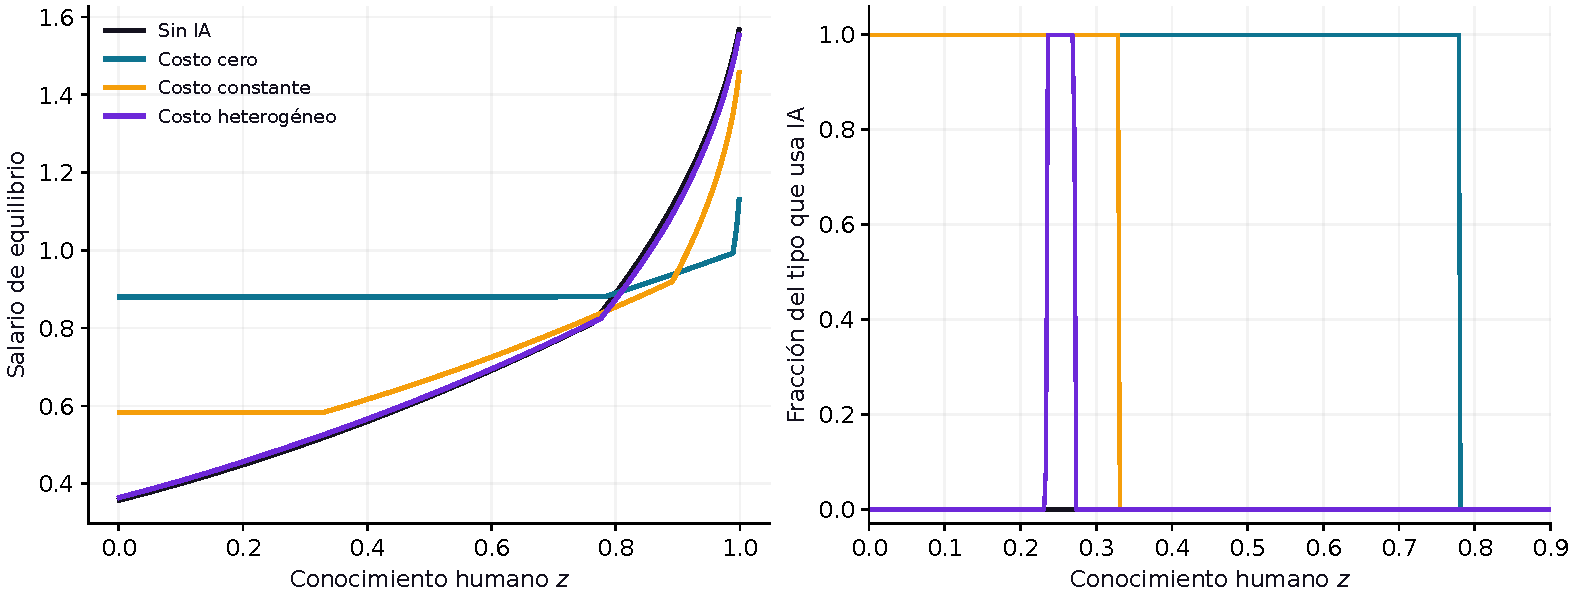
\includegraphics[width=.97\linewidth]{../code/figures/equilibrium.pdf}\end{center}
\begin{center}\small
\begin{tabular}{rrrrr}\toprule
$N$ & $Y^V$ & Masa con IA & Menor $z$ usuario & Mayor $z$ usuario\\\midrule
100&0.692416&0.042187&0.23500&0.27500\\
200&0.692471&0.033137&0.23750&0.27250\\
400&0.692483&0.037226&0.23375&0.27125\\\bottomrule
\end{tabular}
\end{center}
En estas mallas, la fricción heterogénea excluye la base y deja usuarios intermedios. Con costo cero la adopción parte de la base; con costo constante también lo hace, pero su masa es menor. La igualdad salarial $w_i=q_i$ no se utiliza para clasificar usuarios: puede haber tipos indiferentes que no reciben masa de IA.

Los residuos de recursos, no beneficio, complementariedad y brecha primal--dual son menores que $10^{-7}$; el código falla si se supera esa tolerancia. Los CSV guardan los valores efectivos. La estabilidad del producto no debe confundirse con convergencia de masas: estas pasan de $0.0422$ a $0.0331$ y $0.0372$. La aproximación confirma el patrón en mallas concretas, no un teorema del continuo.
\newpage
\section{Discusión, límites y conclusión}\label{sec:discussion}
\subsection{Nivel, pendiente y costo de oportunidad}
Con $c(z)=\bar c$, la oferta $a-\bar c$ es plana. Con $c(z)=\kappa(1-z)$, su pendiente es $\kappa$. A salarios iniciales, $\Delta^{0\prime}=\kappa-w^{0\prime}$, de modo que $\kappa>w^{0\prime}$ indica ventaja de entrada creciente localmente. Esa condición no es suficiente para la Proposición 2: también deben sostenerse las alternativas humanas, los salarios y la capacidad experta. Las desigualdades \eqref{eq:surplus}--\eqref{eq:high} muestran qué añade el cierre de equilibrio.

El costo heterogéneo no domina en bienestar al costo constante de igual promedio. Con $N=400$, el producto neto es aproximadamente $0.692483$ con heterogeneidad y $0.729923$ con costo constante; sin IA es $0.692334$ y sin gasto de validación es $0.893418$. Son comparaciones de tecnologías con costos realizados diferentes. El modelo no permite concluir que una regulación de validación mejore eficiencia o distribución: no incluye daños por errores que dicha regulación pudiera evitar.

\subsection{Fronteras del resultado}
El teorema resuelve un régimen discreto con expertos excedentes. Fuera de esas desigualdades pueden cambiar precios, soporte y ocupaciones. En particular, no se ha probado existencia o unicidad del nuevo equilibrio continuo, ni la convergencia de las mallas al mismo. Tampoco se ha establecido selección intermedia para toda distribución o para cualquier $\kappa>0$. El límite $c=0$ recupera exactamente la tecnología y las restricciones del baseline; las simulaciones muestran su ordenamiento, pero este trabajo no vuelve a demostrar la Proposición 6 del artículo para el continuo.

El gasto es una representación reducida en bienes. Interpretarlo como tiempo del mismo trabajador o de un gerente exigiría cambiar recursos y, posiblemente, $n(z)$. El conocimiento es observable; no hay selección adversa, aprendizaje ni decisiones de educación. La IA no cambia su capacidad y no hay alucinaciones endógenas. Los antecedentes de supervisión estudian otros mecanismos; esta simplificación permite aislar la fricción de costo.

\subsection{Conclusión}
Un costo de validación decreciente puede modificar el acceso efectivo a la IA. El resultado probado construye un equilibrio de tres tipos en el que solo adopta el tipo intermedio, con salarios y recursos determinados dentro del modelo. La base sigue trabajando con expertos humanos. En el continuo uniforme, la resolución sobre tres mallas conserva ese patrón, con residuos verificados y sensibilidad de las masas reconocida.

La diferencia entre una FOC, una oportunidad a precios iniciales y una asignación competitiva es la principal disciplina del ejercicio. El aporte es propio y acotado; no imputa un error al paper base. Las tareas futuras son caracterizar otros regímenes y cerrar el continuo. La autora debe completar la revisión manuscrita y el juicio humano de la asistencia de IA antes de la entrega definitiva del curso.
\label{body:end}
\newpage
\bibliographystyle{plainnat}\bibliography{references}
\newpage\appendix
\section{Asignación finita y certificado de optimalidad}
Para tipos $z_1<\cdots<z_N$, masas $M_i>0$ y $b_i=h(1-z_i)$, el problema primal es
\[
\max_{d,x,y\geq0}\ \sum_i z_i d_i+\sum_{i:z_i\leq a}(a-c_i)x_i+\sum_{i<j}z_jy_{ij},
\]
\[
d_i+x_i+\sum_{j>i}y_{ij}+\sum_{k<i}b_ky_{ki}=M_i,\qquad
x_i=0\text{ si }z_i>a.
\]
Con cómputo abundante su restricción es redundante; se calcula ex post y se exige demanda menor que $\mu$. La variable $y_{ij}$ mide trabajadores, no número de firmas. Se permiten cantidades divisibles, acordes con una población de masa.

El dual minimiza $\sum_iM_iw_i$ sujeto a
\[
w_i\geq z_i,\qquad w_i\geq a-c_i\ (z_i\leq a),\qquad w_i+b_iw_j\geq z_j\ (i<j).
\]
La restricción dual de una actividad es su condición de no beneficio por trabajador. La complementariedad exige igualdad si esa actividad recibe masa positiva. Un primal factible y un dual factible con objetivos iguales certifican optimalidad: multiplicar cada desigualdad dual por la variable primal y sumar utiliza exactamente las restricciones de recursos. Esta es la desigualdad que usa la prueba de unicidad de la Proposición 2; no requiere suponer un equilibrio ya existente.

El primal finito es no vacío (todos independientes), cerrado y acotado: cada variable consume al menos una unidad de alguna masa humana, por lo que está acotada. La programación lineal finita entrega un óptimo y un dual; la existencia finita no resuelve el paso al continuo. El código usa HiGHS mediante SciPy y verifica el certificado sin tomar el estado de éxito del optimizador como único control.

Para el ejemplo exacto, las holguras de actividades no usadas son estrictamente positivas. Los productos netos y sus signos se evalúan con racionales; esa comprobación es independiente de redondeos de la solución LP. Los valores de las tablas se verifican y exportan a CSV, y los gráficos se generan desde \texttt{code/verify.py}; las reglas de tolerancia están en ese único punto de entrada.
\newpage
\section{Formalización Lean y alcance de la verificación}\label{app:lean}
La formalización está en preparación. Se registrarán declaraciones, compilación, commit fuente y cualquier parte abierta. No se atribuye una certificación a archivos aún no comprobados.

\section{Colaboración con IA y adjudicación humana}
La IA asistió en derivación, construcción del certificado, búsqueda bibliográfica, programación y redacción. La autora indicó que el profesor pidió dominar cada derivación. El registro en crudo está en \texttt{prompts.md}; la autora aportó su comprobación y veredicto sobre la cota de $\kappa$; las demás filas siguen siendo controles del asistente, no adjudicaciones humanas.
\begin{center}\small
\begin{tabular}{p{.30\linewidth}p{.24\linewidth}p{.36\linewidth}}\toprule
Afirmación examinada & Estado & Cómo se comprobó\\\midrule
Un borrador de IA exigía $\kappa<1$. & Autora: innecesaria para $c(z)\geq0$. & Comprobación manuscrita real, contraejemplo $\kappa=2$ y veredicto en \texttt{hand/01-revision-kappa.png}.\\[4pt]
$\Delta^0>0$ identifica adoptantes finales. & Incorrecta como regla de equilibrio. & Se resuelve asignación y salarios; se usa masa primal $x_i$.\\[4pt]
La selección intermedia sobrevive en cualquier continuo. & No demostrada. & Solo tres mallas y un teorema de tres tipos.\\[4pt]
El ejemplo de tres tipos es equilibrio. & Certificado por el asistente; revisión humana pendiente. & Prueba completa, racionales y LP independiente.\\\bottomrule
\end{tabular}
\end{center}
\section{Derivaciones de la autora}
La autora proporcionó su comprobación real y su veredicto sobre la no negatividad de $c(z)=\kappa(1-z)$, conservados en \texttt{hand/01-revision-kappa.png} e incorporados en la slide 17. Esta evidencia cubre esa comprobación; no se atribuye a la autora una revisión del resto de los resultados. Las páginas manuscritas sobre derivadas, condición de Fermat, beneficio cero, recursos, holguras y ganancia neta todavía deben incorporarse a \texttt{hand/}. La guía tipográfica ayuda a reconstruirlas, pero no sustituye el trabajo a mano.
\end{document}
